\cotefile{156-8}
\scanpage{90}\mspage{81}
\uline{1 juillet}\qquad \unsure{Magma associé|Magmas associés} à un ensemble ordonné $L$.

\deleted{Je vais \unsure{d}}

A) Supposons d'abord $L$ \uline{totalement} \uline{ordonné}, et \uline{divisible} i.e.
\[
 \forall a,b\in L,\quad a<b\Longrightarrow
 \underbrace{]a,b[}_{\substack{\shortparallel\,\text{déf}\\
     \{x\unsure{\in|\ni}L\mid a<x<b\}}}\ne\varnothing
\]

Dans ce cas, on va définir un \deleted{magma} \uline{\unsure{ens multistr.}}, ayant $L$ comme ens de points (ou lieux), et un
\[
 M\subset\deleted{\unsure{\mathcal P(L)|\mathrm{P}(L)}}\,\unsure{\text{Figél}|\text{Figel}}(L)
\]
défini ainsi\,:
\[
\left\{\begin{aligned}
 &M=M_0\amalg M_1,\quad\text{avec}\\
 &M_0=\big\{\deleted{\unsure{\{\{x\}\}}}\inserted{P_x}\mid x\in L\big\},\quad
     \text{où}\quad \deleted{\unsure{X}}P_x=\{\{x\}\}\\
 &M_1=\{\deleted{\unsure{X}}S_{a,b}\mid a,b\in L,\ a<b\},\quad
     \deleted{\unsure{X}}S_{ab}=\{[a,b],\{a\},\{b\}\}
\end{aligned}\right.
\]
% slanted
\margin{\uline{NB} Quand on écrit $S_{a,b}$, on sous-entend $a<b$. On a besoin de la divisibilité, pour que $S_{a,b}$ soit bien une figure, i.e. \deleted{$S_{a,b}^{\circ}=\unsure{]a,b[}$} $S_{ab}^{\circ}\overset{\text{déf}}{=}|S_{a,b}|\setminus|\partial S_{ab}|\ne\varnothing$}

Il est tautologique que les conditions $\text{Magm }1,2$ sont vérifiées. ($M$ contient les $\{\{x\}\}$ i.e. les $\unsure{X_x|P_x}$, et $M$ stable par passage à une sous-\deleted{\unsure{multi-str}}multistrate.)

Explicitons les relations $\leq,\ \overset{\circ}{\ll},\ |\bullet|$

% slanted
\margin{NB Il vaut mieux utiliser la notation $X\triangleleft Y$ pour $X<Y$ et $X\trianglelefteq Y$ pour $X\leq Y$ (notations d'une relation d'incidence) pour réserver la notation $X<Y$ à la \unsure{rel} ``positionnelle'' $X\underset{\mathrm{pos}}{\leq}Y$. cf p. 97,98.}

\[
\begin{aligned}
1^\circ)\quad X\leq Y\Longleftrightarrow X=Y\ \text{ou}\quad
  X=P_x,Y=S_{a,b},\quad&\text{avec}\quad x\in\{a,b\}\\[-2pt]
 &\text{i.e.}\quad x=a\ \text{ou}\ x=b
\end{aligned}
\]
\[
\deleted{2^\circ)\quad X\overset{\circ}{\ll}Y\quad\text{sss}\quad X=Y\ \text{ou}\ X=P_x,Y}
\]

En d'autres termes, on a
\[
\left\{\begin{aligned}
 \partial P_x&=\varnothing\\
 \partial S_{a,b}&=\{P_a,P_b\}
\end{aligned}\right.
\]

\[
\begin{aligned}
2^\circ)\quad X\overset{\circ}{\ll}Y\Longleftrightarrow{}&
  \deleted{X=Y\ \text{ou}\ \unsure{(}X=P_a,}\\[-2pt]
&\left\{\begin{aligned}
 a)&\ \text{si }X=P_x,Y=P_y:\quad x=y\quad\text{i.e. }P_x=P_y\\
 b)&\ \text{si }X=P_x,\unsure{Y|X}=S_{ab}:\quad a<x<b\quad
       [\text{i.e. }x\in|X|^\circ]\\
 c)&\ \text{si }\unsure{-}X=S_{a,b},\ Y=S_{a',b'}:\quad a'\leq a<b\leq b'\\
   &\qquad[\text{i.e.}\ \unsure{-}\ |X|\subset|Y|,\ \inserted{\text{\deleted{ou} aussi}}\,
                 |X|^\circ\subset|Y|^\circ]
 \end{aligned}\right.
\end{aligned}
\]

On voit donc\({}^{*}\) que les $P_x$ sont les éléments minimaux pour $\leq$, \uline{et} les éléments minimaux pour $\overset{\circ}{\ll}$ (grâce à divisibilité), ce sont donc aussi les él. minimaux pour $\overset{*}{\ll}$ ou lieux
% slanted
\margin{\({}^{*}\) c'est d'ailleurs tout vu, en vertu des \unsure{seules|seuls} a\unsure{.}\deleted{\unsure{xiô}}mes $\text{Magm }1,2$.}
% archive sheet number: 90

\scanpage{91}\mspage{82}
\[
3^\circ)\quad X\,|\circ|\,Y\Longleftrightarrow
 \left\{\begin{aligned}
 X=P_x,Y=P_y:\quad &[x\ne y\ \text{i.e.}]\quad x<y\ \text{ou}\ y<x\\
 X=P_x,Y=S_{a,b}\ (\text{ou l'inverse}):\quad &x\leq a\ \text{ou}\ b\deleted{\unsure{<|>}}\leq x\\
 X=S_{a,b},Y=S_{a',b'}\quad &a<b\leq a'<b'\ \text{ou}\ a'<b'\leq a<b
 \end{aligned}\right.
\]

On a exprimé simplement $|X|^\circ\cap|Y|^\circ\deleted{\unsure{\subset|=}}=\varnothing$, en utilisant la divisibilité.

Dans le contexte ensembliste actuel, on n'a plus d'axiomes à vérifier, pas non plus \deleted{\unsure{des}}d'axiomes du support, grâce à l'existence de la fonction support externe fidèle $X\mapsto|X|$ (comme \deleted{\unsure{chaque}}\inserted{pour} \deleted{\unsure{fois}} tout magma ensembliste, ou simplement ponctuel, voire, seulement fidèle -- en prenant cette fois la fonction support fidèle $X\mathrel{\tikz[baseline=-.45ex,x=1em,y=1em]{\draw (0,0)--(1.15,0) (0,-.10)--(0,.11) (1.15,-.10)--(1.15,.11);}}\unsure{\mathrm{Omb}\,X|\mathrm{Ouvs}\,X|\mathrm{Oens}\,X}$).

B) Supposons maintenant la relation d'ordre quelconque. On prendra encore
\[
\left\{\begin{aligned}
 &M\subset\unsure{\mathcal P|\mathscr P}(\mathcal P(L))\\
 &M=M_0\amalg M_1\\
 &\qquad M_0=\{P_x\mid x\in L\},\qquad P_x=\{\{x\}\}\\
 &\qquad M_1=\{S_{a,b}\mid a,b\in L,\ a<b\}\qquad
 S_{a,b}=\{[a,b],\{a\},\{b\}\},
\end{aligned}\right.
\]
\margin{il \deleted{\unsure{est}} peut-être plus simple de prendre $M_0=L$, $M_1=\{(a,b)\in L\times L\mid a<b\}$}
mais on notera qu'on ne sait pas si $S_{ab}$ est une figure (élémentaire), faute de savoir si
\[
 |S_{a,b}|^\circ=[a,b]\setminus\{a,b\}=]a,b[
\]
\unsure{tjrs|tjous} non vide. On \uline{définira} alors les relations $\leq,\ \overset{\circ}{\ll},\ |\bullet|$ par les formules explicitées plus haut, en faisant attention cette fois que
\margin{\uline{NB} Avec la présentation adoptée, on trouve des ``quasi-figures'' élémentaires \unsure{dans|de} $L$ (on peut avoir $|X|^\circ=\varnothing$) et $\leq,\overset{\circ}{\ll}$ est induit alors, au sens évident, par les notions ensemblistes. Mais \uuline{pas} $|\circ|$, sauf dans le cas tot. ordonné.}
\[
\begin{aligned}
 S_{a,b}\overset{\circ}{\ll}S_{a',b'}\Longleftrightarrow a'\leq a<b\leq b'
 &\ \Longleftrightarrow |S_{a,b}|^{\deleted{\unsure{\circ}}}\overset{\inserted{\unsure{\nRightarrow|\Rightarrow}}}{\subset}|S_{a',b'}|^{\deleted{\unsure{\circ}}}\\
 &\quad\deleted{\text{\unsure{mais l'implication}}}\\
 &\quad\deleted{\text{\unsure{pas nécessairement valable}}}\\
 &\ \Longrightarrow |S_{a,b}|^\circ\subset|S_{a',b'}|^\circ
\end{aligned}
\]
\margin{mais l'implication inverse pas néc. valable}

\[
\deleted{P_x\,|\circ|\,P_y\Longleftrightarrow x<y\ \text{ou}}
\]
% archive sheet number: 91

\scanpage{92}\mspage{83}
\[
 P_x\,|\circ|\,P_y\Longleftrightarrow x<y\ \text{ou}\ y<x\ \text{i.e}\ 
 \{x,y\}\in\unsure{\mathrm{Drap}|\mathrm{Dep}}_2(L)\Longrightarrow x\ne y
\]
\inserted{$\Longleftrightarrow |P_x|^\circ\cap|P_y|^\circ=\varnothing$}
\margin{$\downarrow$ mais l'\unsure{indication|indicition|implication} inverse pas valable en général}
\[
 P_x\,|\circ|\,S_{a,b}\Longleftrightarrow x\leq a\ \text{ou}\ y\geq b
 \Longrightarrow |P_x|^\circ\cap|S_{a,b}|^\circ=\varnothing
\]
\margin{$\hookrightarrow$ mais l'implication inverse pas valable en général}
\[
\begin{aligned}
 S_{a,b}\,|\circ|\,S_{a',b'}&\Longleftrightarrow
 a<b\leq a'<b'\ \text{ou}\ a'<b'\leq a<b\\
 &\Longrightarrow |S_{a,b}|^\circ\cap|S_{a',b'}|^\circ=\varnothing
\end{aligned}
\]
\margin{$\hookrightarrow$ mais implication inverse pas valable en général}
% slanted
\margin{\tikz[baseline]{\node[draw,rounded corners=12pt,text width=2.1cm,inner sep=2pt]{\uline{NB} $X\mathrel{\vcenter{\hbox{\tikz[x=.8em,y=.5em,line join=round]{\draw (0,1)--(1,.5)--(0,0) (1,1)--(0,.5)--(1,0);}}}}Y\Longleftrightarrow X=Y$ ou $X\,|\bullet|\,Y$ chose très spéciale à la dim $1$ \ldots};}}

Cela n'empêche qu'on vérifie directement que \deleted{$\unsure{\notin|\nleq}$} $\leq,\ \overset{\circ}{\ll}$ sont des relations d'ordre, et $|\circ|$ est sym. \unsure{antiréflexive} (Mag 1).

Il faut vérifier Mag 2,3,4.

Mag 2 OK, on trouve de plus
\[
 X\ll Y\Longleftrightarrow\left\{\begin{aligned}
 &X=P_x,Y=P_y,\ x=y\\
 &X=P_x,Y=S_{\unsure{(}a,b},\ 
    \deleted{x\in[a,b](=|S_{a,b}|)}\inserted{a\leq x\leq b}\\
 &X=S_{a,b},Y=S_{a',b'}:\quad a'\leq a<b\leq b',
 \end{aligned}\right.
\]

donc
\[
 \left\{\begin{aligned}
 &X\ll Y\Longleftrightarrow |X|\subset|Y|\\
 &\text{Si}\quad X,Y\in M_1,\quad X\ll Y\Longleftrightarrow X\overset{\circ}{\ll}Y
 \end{aligned}\right.
\]
\[
 \text{Mag }3:\quad X\,|\bullet|\,Y,\ X'\overset{\circ}{\ll}X,\ 
 Y'\overset{\circ}{\ll}Y\Longrightarrow X'\,|\circ|\,Y'\quad\text{OK}
\]
\[
 \text{Mag }4\qquad X\unsure{<|\leq}Y_{\unsure{0|\circ}}\Longrightarrow X\,|\circ|\,Y\quad\text{OK}
\]

Ici encore, les $P_x$ sont \deleted{\unsure{les él}} minimaux à la fois pour $\leq$ et pour $\overset{\circ}{\ll}$. Ce sont les seuls éléments minimaux pour $\leq$, \deleted{en plus il} mais comme éléments minimaux pour $\overset{\circ}{\ll}$, il y a en plus les $S_{a,b}$ tels que $|S_{\unsure{a|x},b}|^\circ=]a,b[=\varnothing$. En tous cas, les lieux sont les $P_x$, l'ens. des lieux s'identifie à $L$.
% archive sheet number: 92

\scanpage{93}\mspage{84}
L'axiome de divisibilité \deleted{\unsure{équi}} Mag L 1. équivaut ici au fait que \deleted{\unsure{la}} l'ens ordonné soit divisible
\[
\begin{aligned}
 \text{Mag L }1&\Longleftrightarrow \forall S_{a,b},\quad |S_{ab}|^\circ\overset{\text{déf}}{=} ]a,b[\ne\varnothing\\
 &\qquad\text{i.e. si }a<b,\ \exists x\ \text{avec}\ a<x<b.
\end{aligned}
\]

Cela implique-t-il Mag L 2 ? \deleted{Non, exemple}

\[
\begin{aligned}
 \substack{\text{Mag L 2 signifie}\\\text{ici deux choses}}\quad
 \left|\begin{aligned}
 a)&\ \text{pour }P_x,S_{a,b}:\quad
     x\parallel\deleted{\unsure{\{} }]a,b[\ \Longrightarrow x\leq a\ \text{ou}\ x\geq b\\
 &\quad\deleted{\Longrightarrow\text{ ou encore }x\parallel\{a,b\}}\\
 b)&\ \text{pour }S_{a,b},S_{a',b'}\quad
      ]a,b[\deleted{\unsure{\bullet}}\mathrel{\unsure{\mid\cdot\mid|\parallel}}]a',b'[
         \Longrightarrow b\leq a'\ \text{ou}\ b'\leq a
 \end{aligned}\right.
\end{aligned}
\]
mais b) résulte en réalité de a) \deleted{\unsure{ou encore}} \deleted{$\Rightarrow\ \unsure{\{a,b\}}\parallel ]a',b'[$, et \unsure{on applique} a)}

\deleted{Dans les deux cas, il faut \unsure{préciser|prouver}}

\uline{Lemme} \deleted{\unsure{Il}}Pour que Mag L 2 soit valable, il f et s. que \inserted{(i) $L$ soit div.} \inserted{et} que \inserted{\deleted{\unsure{(ii)}}} $\forall x\in L$, et $a<b$, on ait
\[
 x\parallel ]a,b[ \Longrightarrow \deleted{x\parallel\{a,b\}} x\leq a\ \text{ou}\ x\geq b.
\]

\deleted{(où pour deux \unsure{parties} une partie $A$ de $L$, on pose}
\[
 \deleted{x\parallel A\Longleftrightarrow\forall y\in A,\quad x\parallel y\quad
         (\text{i.e. } x<y\ \text{ou}\ y<x)}
\]
\deleted{ou encore, que \unsure{s}}
\deleted{a) Si $a\unsure{\notin|\in}L$ n'est pas un plus grand élément, on ait}
\[
 \deleted{L_{\leq a}=\bigcap_{b\in L_{>a}}}
\]

Ou encore, que

\unsure{(iia)|(iii)} a) $\forall a\in L$, t. q. $a$ ne soit pas un plus grand élément, on ait
\[
 \bigcap_{\underset{\sim}{c}>a}L_{\leq c}=L_{\leq a}
\]

b) $\forall b\in L$ tel que $b$ ne soit pas un plus petit élément, on ait
\[
 \bigcap_{\underset{\sim}{c}<b}L_{\geq c}=L_{\geq b}
\]

\unsure{Ce|Ceci} n'est le plus souvent pas satisfait pour les \deleted{\unsure{magmas}} ens. ordonnés associés \deleted{\unsure{aux}}\inserted{à une} corde topologique, exemple
\figure{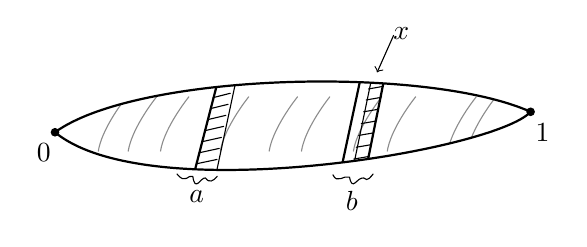
\begin{tikzpicture}[x=1cm,y=1cm,line cap=round,line join=round]
 \begin{scope}
  \clip (0,0) .. controls (1.05,.76) and (4.72,.85) .. (6.04,.26)
       .. controls (5.6,-.23) and (1.19,-.98) .. (0,0);
  \foreach \x in {.70,1.08,1.49,2.25,2.87,3.28,3.94,4.37,5.14,5.39}
     \draw[thin,black!45] (\x-.15,-.24) .. controls (\x-.11,.02) and (\x+.13,.35) .. (\x+.21,.45);
  \draw[thick] (1.71,-.74)--(2.12,.85);
  \draw (2,-.74)--(2.34,.85);
  \foreach \y in {-.53,-.40,-.26,-.12,.02,.16,.30,.44,.58}
     \draw ({1.75+(.59+\y)*.25},\y)--({2.02+(.59+\y)*.20},\y+.055);
  \draw[thick] (3.58,-.72)--(3.91,.82);
  \draw (3.73,-.72)--(4.05,.82);
  \draw[thick] (3.90,-.72)--(4.21,.82);
  \foreach \y in {-.50,-.34,-.19,-.04,.11,.26,.41,.55}
    \draw ({3.74+(.60+\y)*.21},\y)--({3.92+(.60+\y)*.20},\y+.03);
 \end{scope}
 \draw[thick] (0,0) .. controls (1.05,.76) and (4.72,.85) .. (6.04,.26)
       .. controls (5.6,-.23) and (1.19,-.98) .. (0,0);
 \fill (0,0) circle (.055) (6.04,.26) circle (.055);
 \node[below left] at (.07,-.02) {$0$};
 \node[below right] at (5.98,.23) {$1$};
 \draw (1.55,-.53) .. controls (1.66,-.67) and (1.69,-.53) .. (1.75,-.56)
            .. controls (1.78,-.77) and (1.85,-.57) .. (1.91,-.58)
            .. controls (1.96,-.65) and (2.01,-.62) .. (2.06,-.56);
 \node[below] at (1.80,-.62) {$a$};
 \draw (3.53,-.54) .. controls (3.58,-.66) and (3.67,-.54) .. (3.74,-.57)
            .. controls (3.78,-.76) and (3.83,-.57) .. (3.92,-.58)
            .. controls (3.97,-.64) and (4.02,-.55) .. (4.04,-.53);
 \node[below] at (3.77,-.62) {$b$};
 \draw[->] (4.30,1.23)--(4.09,.76);
 \node[above right,inner sep=0pt] at (4.29,1.17) {$x$};
\end{tikzpicture}}
% archive sheet number: 93

\scanpage{94}\mspage{85}
Quand le magma est-il fidèle \unsure{?}\,, I.e. quand a-t-on la condition de fidélité
\begingroup
\makeatletter\tagsleft@true\makeatother
\[
 \mathrm{Omb}^{\circ}(X)\cap\mathrm{Omb}^{\circ}(Y)=\varnothing
 \Longrightarrow X\,|\circ|\,Y\quad ? \tag*{(*)}
\]
\endgroup

Il faut déjà que sur $L$
\[
 P_x\ne P_y\Longrightarrow x\,|\circ|\,y
\]
i.e. que $L$ soit \uline{totalement} ordonné. Cela équivaut à $(*)$ pour $X=P_x$, $Y=P_y$. Dans le cas $X=P_x$, $Y=S_{a,b}$, cela signifie $x\notin ]a,b[\Longrightarrow x\,|\circ|\,S_{ab}$ i.e. $x\leq a$ ou $x\geq b$, OK. Dans le cas où $\deleted{\unsure{x}}X=S_{a,b}$, $Y=S_{a',b'}$, cela signifie que l'on aura \deleted{$S_{a,b}$} si on \deleted{$S_{a,b}$} n'a pas $b\leq\unsure{a'|b'}$ ou $b'\leq a$, i.e. si on a à la fois $\underline{b>a'}$, $\underline{b'>a}$, alors il y a un \unsure{raff} interne commun. Je distingue quatre cas, suivant la position relative de $a$ p.r. à $a'$, et de $b$ p.r. à $b'$

\[
\begin{aligned}
 {}\cdot\quad a'\leq a<b\leq b'&\quad\text{on prend }\deleted{\unsure{[}}S_{ab}\ \text{comme}\\
 &\quad\text{raffinement interne commun}\\[3pt]
 a\leq a'\unsure{<|\leq}b\leq b'\quad\text{ou}\quad a'\leq a<b'\leq b
 &\quad\text{on prend }S_{a'b}\\
 &\qquad\text{resp }S_{ab'}\\[3pt]
 a\leq a'\unsure{<|\leq}b'\leq b&\quad\text{on prend }S_{a',b'}
\end{aligned}
\]

\unsure{Donc|D'où} \uline{Lemme}\qquad $M$ est fidèle sss $L$ est totalement ordonné

\uline{Corollaire}\qquad $M$ est ponctuel sss $L$ est totalement ordonné et divisible (et alors $M$ est \unsure{$=$|un} ens \unsure{multistr.}).
% archive sheet number: 94

\scanpage{95}\mspage{86}
Passons aux questions de \unsure{supports|support}. Dans le cas général, on ne peut se contenter des ombres ou supports \unsure{internes|induits} sur $L$, faute de Mag L 2. \deleted{et même des} D'abord, étudions les figures (finies).
\[
\begin{aligned}
 \deleted{X \mathrel{\vcenter{\hbox{\tikz[x=.8em,y=.5em,line join=round]{\draw (0,1)--(1,.5)--(0,0) (1,1)--(0,.5)--(1,0);}}}} Y}&\left\{\begin{aligned}
 &\deleted{\text{si }X=P_x,Y=P_y:\quad x\unsure{=|\leq|\neq}y\quad\text{\unsure{ou}}\ x\,|\circ|\,y
             \quad\unsure{<x}\quad\text{i.e. }\{x,y\}\in\unsure{\mathrm{Drap}|\mathrm{Drp}}(L)}\\
 &\deleted{\text{si }X=P_x,\ Y=S_{a,b}:\quad\text{si }x\ll S_{ab}\ \text{i.e. }x\notin[a,b]:
                x\parallel S_{ab}}\\
 &\deleted{x\in\{a,b\}\quad\text{\uline{ou}}\quad x\parallel}
 \end{aligned}\right.
\end{aligned}
\]

\deleted{\unsure{R}}Examinons la condition de compatibilité $X \mathrel{\vcenter{\hbox{\tikz[x=.8em,y=.5em,line join=round]{\draw (0,1)--(1,.5)--(0,0) (1,1)--(0,.5)--(1,0);}}}} Y$. Si $X$ disons \unsure{(ou $Y$)|($Y$)} est de la forme $P_x$, donc un lieu
\[
 \begin{aligned}
 P_x \mathrel{\vcenter{\hbox{\tikz[x=.8em,y=.5em,line join=round]{\draw (0,1)--(1,.5)--(0,0) (1,1)--(0,.5)--(1,0);}}}} \deleted{\unsure{X}}Y_{\unsure{a|\epsilon|{}}}
   &\Longleftrightarrow P_x=Y\ \text{ou}\ 
      \underbrace{P_x\,|\circ|\,Y}_{\deleted{\text{donc }\{x,y\}\in\unsure{\mathrm{Dr}}}}\\
   &\hspace{1em}\unsure{:}
 \end{aligned}
\]
\margin{(vrai pour tout lieu dans un magma}

\deleted{donc}
\[
\begin{aligned}
 P_x \mathrel{\vcenter{\hbox{\tikz[x=.8em,y=.5em,line join=round]{\draw (0,1)--(1,.5)--(0,0) (1,1)--(0,.5)--(1,0);}}}} P_y&\Longrightarrow\{x,y\}\in \mathrm{Drap}(L)\\
 P_x \mathrel{\vcenter{\hbox{\tikz[x=.8em,y=.5em,line join=round]{\draw (0,1)--(1,.5)--(0,0) (1,1)--(0,.5)--(1,0);}}}} S_{a,b}&\Longleftrightarrow P_x\,|\bullet|\,S_{ab}
              \Longleftrightarrow x\leq a\ \text{ou}\ \unsure{x|a}\geq b
\end{aligned}
\]

D'autre part, $S_{ab} \mathrel{\vcenter{\hbox{\tikz[x=.8em,y=.5em,line join=round]{\draw (0,1)--(1,.5)--(0,0) (1,1)--(0,.5)--(1,0);}}}} S_{a',b'}$ signifie que, ou bien $S_{ab}=S_{a',b'}$, ou bien $S_{ab}\parallel S_{a',b'}$, ou \deleted{$\unsure{\widetilde S|S}$} $\widetilde S_{a,b}\cap\widetilde S_{a',b'}$ contenu dans $\partial S_{a,b}\cap\partial S_{a',b'}^{\unsure{+|*}}$ et non vide. \inserted{\uline{et} $S_{ab}\,|\circ|\,S_{a',b'}$}

Dans ce dernier cas, je dis que l'intersection \inserted{$\partial S\cap\partial S'$} est réduite à un \inserted{seul} \deleted{point} élément -- s'il y en avait deux, on aurait en effet $\partial S=\partial S'$, d'où $S=S'$, cas que nous avions exclu. On trouve ainsi
\[
 \text{\unsure{la}}\quad S_{a,b} \mathrel{\vcenter{\hbox{\tikz[x=.8em,y=.5em,line join=round]{\draw (0,1)--(1,.5)--(0,0) (1,1)--(0,.5)--(1,0);}}}} S_{a',b'}\Longleftrightarrow
 \left\{\begin{aligned}
 &\text{ou}^{\text{(i)}}\ S_{a,b}=S_{a',b'}\quad\text{i.e }a=a',b=b'\\
 &\text{ou}^{\text{(ii)}}\ S_{a,b}\,|\unsure{\bullet|\circ}|\,S_{a',b'},\
       \deleted{\text{\unsure{ou}}}\ \text{i.e }a<b<a'<b'\ \text{ou}\ a'<b'<a<b\\
 &\text{ou}^{\text{(iii)}}\ a<b\deleted{\unsure{<}}\unsure{\leq|=}a'<b'
                   \quad\text{ou}\ a'<b'\leq a<b\\
 &\quad\deleted{\text{\unsure{ou bien}}}\\
 &\quad\deleted{\text{i.e. }S_{ab}\,|\circ|\,S_{a',b'}}\\
 &\quad\deleted{\text{(mais alors encore } S_{a,b}\,|\circ|\,S_{a',b'}}
 \end{aligned}\right.
\]
au total
\[
\begin{aligned}
 S_{a,b} \mathrel{\vcenter{\hbox{\tikz[x=.8em,y=.5em,line join=round]{\draw (0,1)--(1,.5)--(0,0) (1,1)--(0,.5)--(1,0);}}}} S_{a',b'}&\Longleftrightarrow S_{a,b}=S_{a',b'}\ \text{ou}\ S_{a,b}\,|\circ|\,S_{a',b'}\\
 &\qquad\deleted{\text{i.e. } a<}\\
 &\qquad\text{ce dernier cas s'écrivant}\\
 &\qquad a<b\leq a'<b'\ \text{ou}\ a'<b'\leq a<b
\end{aligned}
\]
% archive sheet number: 95

\scanpage{96}\mspage{87}
Posons
\[
 \delta X=\left\{\begin{aligned}
 &\unsure{x|X}\ \text{si }\deleted{\unsure{x}}X=P_x\\
 &|\partial X|=\{a,b\}\ \text{si }X=S_{a,b}
 \end{aligned}\right.
\]
donc en tous cas
\[
 \delta X\subset L,\qquad \unsure{\operatorname{card}|\operatorname{Card}}\delta X\in\{1,2\}
\]

\deleted{Soient} Une condition \uline{nécessaire} pour $X \mathrel{\vcenter{\hbox{\tikz[x=.8em,y=.5em,line join=round]{\draw (0,1)--(1,.5)--(0,0) (1,1)--(0,.5)--(1,0);}}}} Y$ est
\[
\begin{aligned}
 X \mathrel{\vcenter{\hbox{\tikz[x=.8em,y=.5em,line join=round]{\draw (0,1)--(1,.5)--(0,0) (1,1)--(0,.5)--(1,0);}}}} Y\Longrightarrow\delta(\unsure{x|X})\cup\delta(Y)\in
  \underset{\inserted{\substack{\text{ens des parties}\\\text{finies }\deleted{\unsure{to}}\text{tot. ord de }L.}}}
            {\underline{\mathrm{Drap}(L)}}
\end{aligned}
\]

\deleted{\unsure{cette}} ce drapeau peut avoir cardinal égal à $1$. (si $X=Y\in M_0$), $2,3$, ou $4$ (si $X,Y\in M_1$ et $X\parallel Y$). Le cas de cardinal $2$ est celui de $P_{\unsure{a|x}} \mathrel{\vcenter{\hbox{\tikz[x=.8em,y=.5em,line join=round]{\draw (0,1)--(1,.5)--(0,0) (1,1)--(0,.5)--(1,0);}}}} P_y$ avec $x\ne y$, ou de $P_x \mathrel{\vcenter{\hbox{\tikz[x=.8em,y=.5em,line join=round]{\draw (0,1)--(1,.5)--(0,0) (1,1)--(0,.5)--(1,0);}}}} S_{a,b}$ avec $P_x\triangleleft S_{ab}$ i.e. $x\in\{a,b\}$, ou $\deleted{\unsure{S}}X=Y\in\deleted{\unsure{S}}M_1$\,; le cas de cardinal $3$ est $X\in M_0$, $Y\in M_1$ ou inversement, avec $X\parallel Y$ (soit $P_x,S_{a,b}$ avec $x<a$ ou $\unsure{x|a}>b$), ou celui de $X,Y\in M_1$, placés comme $\deleted{\unsure{S_{a,}}}\ S_{a,b},S_{b,c}$ avec $a<b<c$ -- (segments \uline{contigus}). Soit tabl. possibilités
\diagram{\(\displaystyle
 \left\{\begin{array}{@{}l@{}}
 \text{lieux égaux ou }\deleted{\text{\unsure{intérieurement}}}\ \text{disjoints}\\
 \text{lieu }\deleted{\text{adjacent}}\ \text{incident à un segment, ou disjoint du}\\
 \hspace{17em}\text{segment}\\
 \text{segments disjoints, segments adjacents}
 \end{array}\right.
\)}

Mais de façon générale, si on a $T\in\mathrm{Drap}(L)$,
\[
 T=\{t_1,t_2,\ldots,t_{\unsure{n|m}}\}\quad\text{avec}\quad t_1<t_2<\ldots<t_n,
\]
on \unsure{définit|définira} les \uline{segments} \uline{interstitiels} \inserted{de $T$} comme segments $\deleted{\unsure{P}}S_{t_1,t_2},S_{t_2,t_3},\ldots S_{t_{n-1},t_n}$. \deleted{Ceci}\inserted{les} \deleted{dit, on trouve ceci.} $P_{t_i}$ sont appelés les \uline{lieux} interstitiels. Ceci dit, on trouve ceci\,:
% slanted
\margin{\uline{NB} Si $\operatorname{card}T=1$, il n'y a pas \unsure{de segment interstitiel|de segments interstitiels}, \unsure{seult} \uline{un} lieu interstitiel}
% archive sheet number: 96

\scanpage{97}\mspage{88}
\uline{Proposition} Soit $F\subset M$ une partie finie \inserted{non \unsure{vide|vides}} de $M$, posons $\deleted{\unsure{\delta}}\delta F=\bigcup_{X\in F}\delta X$. Pour que $F$ soit formé de multistrates mutuellement compatibles, il f et s. que les deux conditions suivantes soient satisfaites
% slanted
\margin{\deleted{\unsure{On|(On} appellera ces parties les parties}}
\[
 \text{(i)}\quad\delta F\in\mathrm{Drap}(L)
 \qquad\deleted{[\text{NB }\delta F=\varnothing\ \text{sss}\ F=\varnothing]}
\]
(ii) Les éléments de $F$ sont interstitiels pour $\delta F$.

Dém. par récurrence sur $\operatorname{card}F$. \deleted{On \unsure{voit} que} Pour un $\deleted{\unsure{\delta F}}\inserted{T\in\mathrm{Drap}(L)}$ donné, il y a donc une partie de $M$ \deleted{$X \mathrel{\vcenter{\hbox{\tikz[x=.8em,y=.5em,line join=round]{\draw (0,1)--(1,.5)--(0,0) (1,1)--(0,.5)--(1,0);}}}} Y\ \unsure{=}$} \unsure{maximale}, parmi les parties \deleted{\unsure{figures|form}} formées d'élé. mut. compatibles et telle que $\delta F=T$\,:\ \unsure{à savoir}\ $\unsure{\lceil|\Gamma|F}$
\[
 \begin{aligned}
 F_T={}&\text{\unsure{ensemble|l'ensemble} de toutes les strates interstitielles}\\
 &\text{de }T.
 \end{aligned}
\]
On l'appellera la \uline{figure} \uline{canonique} définie par $T$.

\deleted{Considérons maintenant le cas le plus simple (à part celui où $\operatorname{card}T=1$) celui de}
\[
 \deleted{F=\widetilde S_{a,b}=\{S_{a,b},P_a,P_b\}.}
\]
\deleted{On considère les \deleted{quatre supports} trois supports}
\[
 \deleted{\deleted{\unsure{P}}S_a=\mathrm{supp}^{\circ}P_a,\quad
         \deleted{\unsure{P}}S_b=\mathrm{supp}^{\circ}\deleted{\unsure{S}}P_b,\quad
         \deleted{\unsure{P}}S_{\unsure{\xi|c}}=\mathrm{supp}^{\circ}S_{a,b}.}
\]
\deleted{\unsure{La question} \deleted{\unsure{Il y a}} des supports concerne une subdivision de cet ens de trois éléments, en deux paquets. Il y a \unsure{essentiellement|essentiellemt} \deleted{\unsure{trois}}deux cas \unsure{distincts} non triviaux}
% archive sheet number: 97

